\documentclass{beamer}

\usepackage{beamerthemesplit}
\usepackage{verbatim}

%\definecolor{MyGreen}{RGB}{60, 140, 60}
\definecolor{DarkPurple}{RGB}{60, 30, 60}
\definecolor{Gray90}{RGB}{230, 230, 230}
\definecolor{Gray10}{RGB}{25, 25, 25}


\usetheme{Pittsburgh}
%\usecolortheme{seagull}
%\usecolortheme{spruce}
%\usecolortheme{seahorse}
%\usecolortheme{beaver}
\setbeamercolor{structure}{fg=DarkPurple!90!black}
%\setbeamercolor{structure}{fg=Gray10!10!DarkPurple}

\usefonttheme{serif}

%\DeclareGraphicsExtensions{.pdf,.png,.jpg}

\newcommand{\snT}{$(S/N)_{\textrm{size}}$}
%\newcommand{\snT}{$\left( \frac{S}{N}\right)_{\textrm{size}}$}
\newcommand{\snflux}{$(S/N)_{\textrm{flux}}$}
%\newcommand{\snflux}{$\left( \frac{S}{N}\right)_{\textrm{flux}}$}

\newcommand{\lensfit}{\texttt{LENSFIT}}
\newcommand{\numba}{\texttt{Numba}}
\newcommand{\python}{\texttt{Python}}
\newcommand{\shear}{{\bf g}}

\newcommand{\ngmix}{{\bf ngmix}}
\newcommand{\imshape}{{\bf im3shape}}


% http://texblog.net/latex-archive/plaintex/beamer-footline-frame-number/
% to add the page (frame ) number and not screw up the bottom line
% works for split themes?
\expandafter\def\expandafter\insertshorttitle\expandafter{%
      \insertshorttitle\hfill%
        \insertframenumber\,/\,\inserttotalframenumber}

% suppress navigation bar
\beamertemplatenavigationsymbolsempty

\begin{document}

%\frame{\titlepage}

%\section{DES Shear Pipelines}

\title{DES Shear Pipelines}
\author{Erin Sheldon}
\institute{Brookhaven National Laboratory \newline {\tiny (For the Shear Pipeline \& Testing Subgroup)}}
\date{DES Collaboration Meeting, Sussex, 2014-10-20 }

\frame{\titlepage}

\frame
{
    \frametitle{Outline}

    \begin{itemize}

        %\item Brief description of the data and pipelines.
        \item Brief description of the two pipelines.
        \item Systematics tests
            \begin{itemize}
                \item PSF tests
                \item Shear tests: simulation
                \item Shear tests: null tests on data (SVA1)

                \item Many tests had to be left out due to time constraints:
                    try to focus on the simplest to demonstrate.

            \end{itemize}
        \item Summary
    \end{itemize}
}
 
\frame
{
    \frametitle{Pipelines}

    %\fontsize{9}{0.8\baselineskip}

    \begin{itemize}
        \item \imshape: maximum likelihood fitter (Zuntz et al.)
            \begin{itemize}
                \item Known to be biased: correct for biases using sims.
                \item Single band
            \end{itemize}
        \item \ngmix: bayesian shear estimation (Sheldon)
            \begin{itemize}
                \item Less biased, but more computationally expensive $(\sim 2.5)$
                \item Fit all bands at simultaneously
            \end{itemize}

        \item Multi-epoch
            fitting using Multi-Epoch Data Structures. Collect all postage
            stamps from all single-epoch data into one file per tile.
            \url{https://cdcvs.fnal.gov/redmine/projects/deswlwg/wiki/Multi_Epoch_Data_Structure}

        %\item Algorithms are run on all epochs simultaneously: PSF is
        %    better behaved and understood on the single-epoch images.

        %\item We use Multi-Epoch Data Structures for our processing (MEDS).
        %    MEDS files include:
        %    \begin{itemize}
        %        \item all postage stamps from all epochs associated with
        %            each coadd object.
        %        \item weight maps
        %        \item bit masks
        %        \item other metadata
        %    \end{itemize}

        %\item We only use coadds for detection.

    \end{itemize}
}

\frame
{
    \frametitle{PSF Measurement}

    \fontsize{9}{0.8\baselineskip}

    \begin{columns}
        \begin{column}{0.45\textwidth}
            \begin{itemize}

                \item We use PSFEx (Bertin) to model the PSF and interpolate it to
                    the locations of galaxies.

                \item Errors translate directly into galaxy shapes.

                \item $\rho$-statistics tell us about the spatial correlation 
                    of errors in the PSF modeling.

                \item $\rho_1$ is the auto-correlation of the residuals between
                    the measured shape of stars and that of the interpolated PSF.
                    $\langle \delta e \delta e\rangle$
                \item $\rho_2$ is the correlation of the shape with the residuals
                    $\langle e \delta e\rangle$

                \item Figures: Mike Jarvis

            \end{itemize}
        \end{column}
        \begin{column}{0.55\textwidth}

            \begin{center}
                \includegraphics[width=0.8\textwidth]{rho1-psfex-crop.pdf}
                \newline
                \includegraphics[width=0.8\textwidth]{rho2-psfex-crop.pdf}
                \newline


            \end{center}
        \end{column}
    \end{columns}

}

\frame
{
    \frametitle{Calibration Errors: Noise Bias}

    \begin{itemize}

        \item Using point estimates for shear can result in ``noise bias'', a
            calibration error that depends on S/N.

        \item GREAT DES simulations were created to test noise bias (Kacprzak).
            Cannot test absolute calibration with data.

        \item \imshape:  measure noise bias and correct for it.

        \item \ngmix: no detectable noise bias

    \end{itemize}

    \begin{center}
        \includegraphics[width=0.5\textwidth]{noise-bias-im3shape.png}
        \includegraphics[width=0.5\textwidth]{noise-bias-ngmix.png}
    \end{center}
    {\tiny (Figures: Tomasz Kacprzak)}
}

\frame
{
    \frametitle{Calibration Errors: Apples to Apples}

    \fontsize{9}{0.8\baselineskip}
    \begin{itemize}

        \item Average signal from RedMapper clusters

        \item \imshape\ vs. \ngmix\ using matched source list

        
        %\item To leading order, this test is independent of photoz errors:
        %    \begin{itemize}
        %        \item different weighting can lead to different photoz errors
        %    \end{itemize}

                %\begin{itemize}
                %    {\tiny
                %    \item \imshape\ higher at the $\sim$ 10\% level.

                %    \item Maybe different weighting $\leftrightarrow$ different photoz errors: $(S/N)_{im3}=20 \leftrightarrow (S/N)_{ngmix}=40$
                %    }
                %\end{itemize}
    \end{itemize}

    \begin{center}
        %\includegraphics[width=0.4\textwidth,angle=-90]{dsig_compare_crop.pdf}
        \includegraphics[width=0.35\textwidth,angle=-90]{dsig_ratio_crop.pdf}
    \end{center}
    {\tiny Figure: Andres Plazas
        For more details see talk in cluster lensing
            session Tues. 15:45
        }
}


\frame
{
    \frametitle{PSF Leakage}

    PSF Correction: Look for correlation between galaxy shape and PSF shape.

    \begin{columns}
        \begin{column}{0.38\textwidth}
            \begin{center}
                \includegraphics[width=\textwidth]{im3shape-PSF-E2.pdf}
                \newline
                {\tiny Figure: Vinu Vikram (\imshape)}
            \end{center}
        \end{column}
        \begin{column}{0.62\textwidth}
            \begin{center}
            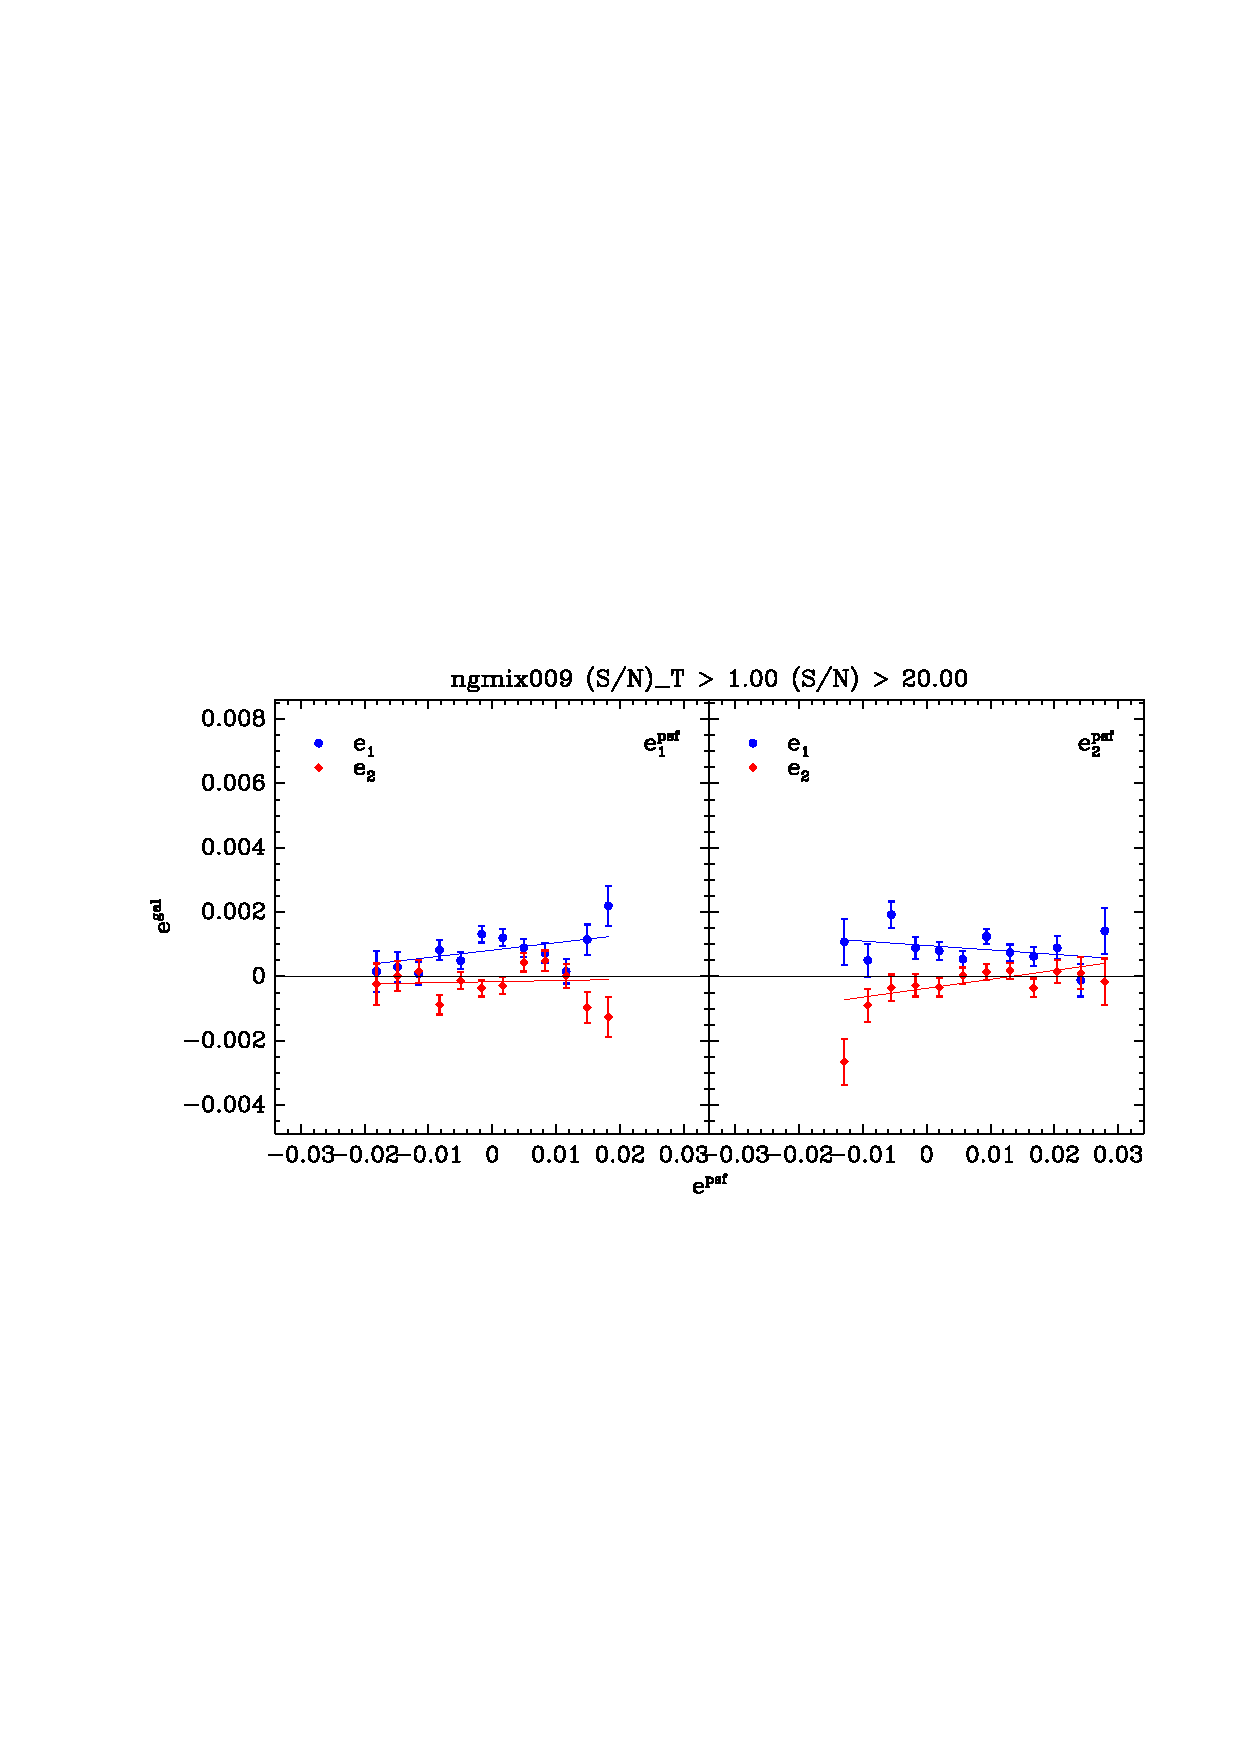
\includegraphics[width=\textwidth]{ngmix009-e-vs-epsf-Ts2n-min-1-s2n-min-20.pdf}
                \newline
                {\tiny Figure: Erin Sheldon}
            \end{center}
        \end{column}
    \end{columns}
}

\frame
{
    \frametitle{PSF Leakage}

    \begin{columns}
        \begin{column}{0.38\textwidth}
            \begin{center}
                \includegraphics[width=\textwidth]{im3shape-PSF-E1.pdf}
                \newline
                {\tiny Figure: Vinu Vikram (\imshape)}
            \end{center}
        \end{column}
        \begin{column}{0.62\textwidth}
            \begin{center}
            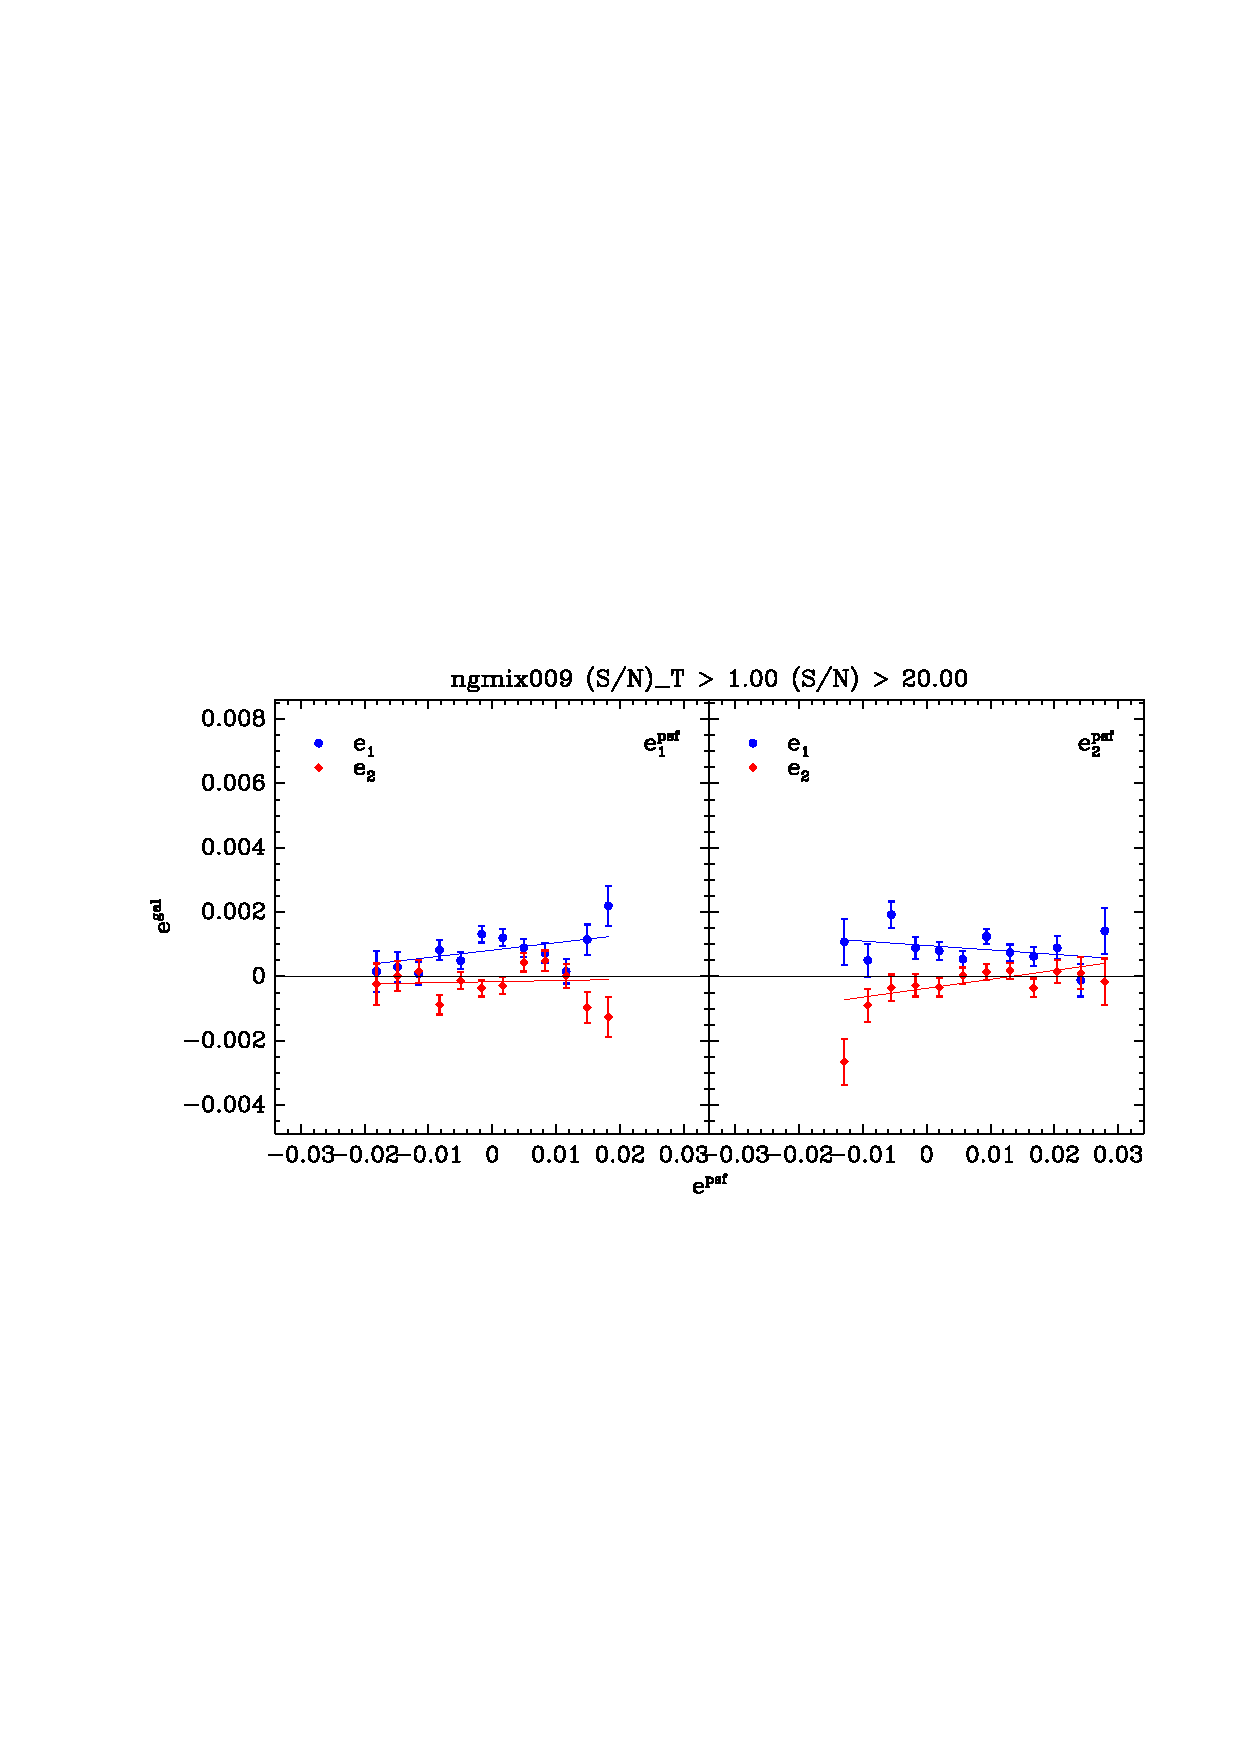
\includegraphics[width=\textwidth]{ngmix009-e-vs-epsf-Ts2n-min-1-s2n-min-20.pdf}
                \newline
                {\tiny Figure: Erin Sheldon}
            \end{center}
        \end{column}
    \end{columns}
}


\frame
{
    \frametitle{Shear Around Stars}

    Look for spurious signal round stars

    \begin{center}
        \includegraphics[width=0.7\textwidth]{star_gal_cs85_m16-22.pdf}
    \end{center}
    {\tiny Figure: Niall Maccrann (im3shape)}
}


\frame
{
    \frametitle{Random Points}

    Look for spurious signal round random points

    \begin{center}
        \includegraphics[width=0.7\textwidth]{random_points_im3shape_ngmix.pdf}
    \end{center}
    {\tiny Figure: Carles S\`{a}nchez}
}

\frame
{
    \frametitle{B Modes}

    \fontsize{9}{0.8\baselineskip}
    \begin{itemize}

        \item Gravity only produces an E mode shear (shears transform like
            polarizations).

        \item B mode should be consistent with zero.

        \item B mode estimation (Becker \& Rozo, in prep).

            \begin{itemize} 

                {\tiny 
                    \item Every other point $\sim$ independent.
                    \item No bayesian sensitivities applied for ngmix, which will boost the signal
                    }

            \end{itemize} 

        \item These data are {\bf blinded}.

    \end{itemize}

    \begin{columns}

        \begin{column}{0.5\textwidth}
            \begin{center}
                \includegraphics[width=1.05\textwidth]{im3shape_v7_r_crop.pdf}
            \end{center}
        \end{column}

        \begin{column}{0.5\textwidth}
            \begin{center}
                \includegraphics[width=1.05\textwidth]{ngmix009_eb_crop.pdf}
            \end{center}
        \end{column}

    \end{columns}
    {\tiny Figures: Matt Becker}
}

\frame
{
    \frametitle{Unexplained Systematics}

    \begin{itemize}

        \item Most of the null tests look good, but there are a few unexplained
            correlations.

        \item Measured galaxy shape correlates with the size of the postage stamp
    
         \item Measured galaxy shape correlates with the fraction of the stamp
             not used for measurement, a.k.a the {\em masked fraction}.

     \end{itemize}

    \begin{center}
        \includegraphics[width=0.5\textwidth]{im3shape-v-vs-mask-frac.png}
    \end{center}

     {\tiny Figure: Vinu Vikram (\imshape)}
}

\frame
{
    \frametitle{Summary}

    \begin{itemize}

        \item PSF $\rho$-statistics may be good enough for SVA

        \item Calibrations of \imshape\ and \ngmix\ very similar for a low number
            density subset of common sources

        \item Most of the shear null tests look good.

            \begin{itemize}

                \item There are still some unexplained correlations.  Still working
                    on the best way to mitigate these effects.

            \end{itemize}
            
        \item Optimistic we will be ready for SVA1 science before year end.

    \end{itemize}
}


\frame
{
    \frametitle{Extra Slides}
    {\Huge Extra Slides}
}


\end{document}
